\documentclass{article}

% if you need to pass options to natbib, use, e.g.:
% \PassOptionsToPackage{numbers, compress}{natbib}
% before loading nips_2018

% ready for submission
\usepackage{nips_2018}

% to compile a preprint version, e.g., for submission to arXiv, add
% add the [preprint] option:
% \usepackage[preprint]{nips_2018}

% to compile a camera-ready version, add the [final] option, e.g.:
% \usepackage[final]{nips_2018}

% to avoid loading the natbib package, add option nonatbib:
% \usepackage[nonatbib]{nips_2018}

\usepackage[utf8]{inputenc} % allow utf-8 input
\usepackage[T1]{fontenc}    % use 8-bit T1 fonts
\usepackage{hyperref}       % hyperlinks
\usepackage{url}            % simple URL typesetting
\usepackage{booktabs}       % professional-quality tables
\usepackage{amsfonts}       % blackboard math symbols
\usepackage{nicefrac}       % compact symbols for 1/2, etc.
\usepackage{microtype}      % microtypography
\usepackage{amsmath}
\usepackage{amssymb}
\usepackage{xcolor}
\usepackage[active]{srcltx}

\usepackage[algo2e,inoutnumbered,algoruled,vlined]{algorithm2e} %linesnumbered
\usepackage{wrapfig}
\usepackage{mathtools}



% \newcommand{\W}{{\cal W}_2}
% \newcommand{\F}{{\cal F}}
% \newcommand{\He}{{\cal H}}
% \newcommand{\SW}{{\cal S}{\cal W}_2}

% \DeclareMathOperator*{\argmin}{arg\min}

\newcommand{\x}{\mathbf{x}}
\newcommand{\thb}{\mathbf{x}} 
\newcommand{\Ths}{{\cal X}} 
% \newcommand{\thb}{\boldsymbol{\theta}} 
% \newcommand{\Ths}{{\cal M}} 
\newcommand{\xe}{\tilde{\mathbf{x}}} 

\newcommand{\B}{\mathcal{B}}
\newcommand{\N}{\mathcal{N}}
\newcommand{\q}{\mathbf{q}}
\newcommand{\qc}{\mathbf{\bar{q}}}
\newcommand{\p}{\mathbf{p}}
\newcommand{\tb}{\mathbf{t}} 
\newcommand{\Ds}{{\cal D}} 

\newcommand{\M}{\mathbf{M}}
\newcommand{\stl}{l}
\newcommand{\Lo}{{\cal L}}
\newcommand{\Oc}{{\cal O}}
\newcommand{\Lot}{\tilde{\Lo}}
\newcommand{\y}{\mathbf{y}}
\newcommand{\Y}{{ Y}}
\newcommand{\D}{ {\cal D} }
\newcommand{\ba}[1]{b(#1,\alpha)}
\newcommand{\bta}[1]{\tilde{b}_{h,K}(#1,\alpha)}
\newcommand{\bha}[1]{\hat{b}(#1,\alpha)}
\newcommand{\rmd}{r}
\newcommand{\Sp}{\mathbb{S}}
\newcommand{\R}{\mathbb{R}}
\newcommand{\E}{\mathbb{E}}
\newcommand{\Pro}{\mathbb{P}}
\newcommand{\Pb}{\mathbf{P}}
\newcommand{\overbar}[1]{\mkern 1.5mu\overline{\mkern-1.5mu#1\mkern-1.5mu}\mkern 1.5mu}

\newcommand{\W}{{\cal W}_2}
\newcommand{\F}{{\cal F}}
\newcommand{\PS}{{\cal P}}
\newcommand{\He}{{\cal H}}
\newcommand{\SW}{{\cal S}{\cal W}_2}
\newcommand{\TV}{\textnormal{TV}}
\newcommand{\KL}{\textnormal{KL}}
\newcommand{\muh}{\hat{\mu}}

\newtheorem{thm}{Theorem}
\newtheorem{remark}{Remark}
\newtheorem{cor}{Corollary}
\newtheorem{lemma}{Lemma}
\newtheorem{prop}{Proposition}

\DeclareMathOperator*{\argmin}{arg\min}
\DeclareMathOperator*{\argmax}{arg\max}

\DeclareMathOperator{\cB}{\overline{B}}


\newcommand{\tmpeqno}{{\color{red} (TEMPEQ) }}

\newcommand{\umut}[1]{{\color{red} (#1)} }

\DeclareMathOperator{\sign}{sign}
\newcommand{\sas}{{\cal S} \alpha {\cal S} }

% \newcommand{\pb}{\bar{{\cal P}}}
% \newcommand{\pt}{\tilde{{\cal P}}}

\newcommand{\pb}{{\cal P}^\x}
\newcommand{\pt}{{\cal P}^\y}

% \newcommand{\ab}{\bar{{\cal A}}}
% \newcommand{\at}{\tilde{{\cal A}}}

\newcommand{\ab}{{\cal A}^\x}
\newcommand{\at}{{\cal A}^\y}

\usepackage{cleveref}


% \newtheoremstyle{exampstyle}
%   {\topsep} % Space above
%   {0} % Space below
%   {} % Body font
%   {} % Indent amount
%   {\bfseries} % Theorem head font
%   {.} % Punctuation after theorem head
%   {0pt} % Space after theorem head
%   {} % Theorem head spec (can be left empty, meaning `normal')

% \theoremstyle{exampstyle} 

\newtheorem{assumption}{\textbf{H}\hspace{-3pt}}
\Crefname{assumption}{\textbf{H}\hspace{-3pt}}{\textbf{H}\hspace{-3pt}}
\crefname{assumption}{\textbf{H}}{\textbf{H}}



\newcommand{\insertimage}[4]{ % scale, filename, caption, label
\begin{figure}[t]
\centering
\includegraphics[scale=#1, clip=true]{figures/#2}
\caption{#3}
\label{#4}
\end{figure}
}

\newcommand{\insertimageC}[5]{ % scale, filename, caption, label, location
\begin{figure}[#5]
\centering
\includegraphics[width=#1\linewidth, clip=true]{figures/#2}
%\vspace{-1.5em}
\caption{#3}
%\vspace{-0.5em}
\label{#4}
\end{figure}
}

%\setlength{\belowcaptionskip}{-10pt}
%\captionsetup[figure]{calcwidth = 0.95\linewidth,skip=10pt}
% \setlength{\abovecaptionskip}{-10pt}

\newcommand{\insertimageStar}[5]{ % scale, filename, caption, label, location
\begin{figure*}[#5]
\centering
\includegraphics[width=#1\linewidth, clip=true]{figures/#2}
\caption{#3}
%\vspace{-0.5em}
\label{#4}
\end{figure*}
}

\newcommand{\insertimageAsSubfig}[5]{ % scale, filename, caption, label,
\begin{figure}[#5]
\begin{center}
\subfigbottomskip =-4in
\subfigure{
\includegraphics[width=#1\columnwidth]{figures/#2}
\label{#4}
}
\end{center}
\subfigbottomskip =-4in
\caption{#3}
\label{#4}
\end{figure}
}


\newcommand{\floor}[1]{\left\lfloor #1 \right\rfloor}
\newcommand{\ceil}[1]{\left\lceil #1 \right\rceil}


\title{Sliced-Wasserstein Flows: Nonparametric Generative Modeling via Optimal Transport and MCMC} 
% Learning Transportation Maps via MCMC with Provable Guarantees

% The \author macro works with any number of authors. There are two
% commands used to separate the names and addresses of multiple
% authors: \And and \AND.
%
% Using \And between authors leaves it to LaTeX to determine where to
% break the lines. Using \AND forces a line break at that point. So,
% if LaTeX puts 3 of 4 authors names on the first line, and the last
% on the second line, try using \AND instead of \And before the third
% author name.

\author{
  David S.~Hippocampus\thanks{Use footnote for providing further
    information about author (webpage, alternative
    address)---\emph{not} for acknowledging funding agencies.} \\
  Department of Computer Science\\
  Cranberry-Lemon University\\
  Pittsburgh, PA 15213 \\
  \texttt{hippo@cs.cranberry-lemon.edu} \\
  %% examples of more authors
  %% \And
  %% Coauthor \\
  %% Affiliation \\
  %% Address \\
  %% \texttt{email} \\
  %% \AND
  %% Coauthor \\
  %% Affiliation \\
  %% Address \\
  %% \texttt{email} \\
  %% \And
  %% Coauthor \\
  %% Affiliation \\
  %% Address \\
  %% \texttt{email} \\
  %% \And
  %% Coauthor \\
  %% Affiliation \\
  %% Address \\
  %% \texttt{email} \\
}



\begin{document}
% \nipsfinalcopy is no longer used

\maketitle

\begin{abstract}
We do generative modeling with sliced-Wasserstein flows. 
\end{abstract}


%!TEX root = ./nips_2018_sketchmcmc.tex

\section{Introduction}

% \begin{itemize}
% \item Short intro to implicit generative models
% \item Connection with optimal transport \cite{genevay2017gan}, several other papers
% \item Information about sliced-Wasserstein distance and usage in generative modeling \cite{bonnotte2013unidimensional,kolouri2018sliced,wu2017generative}
% \item Contributions of the current paper
% \begin{itemize}
% \item Development of a novel gradient flow for generative modeling purpose
% \item Establish the connections with SDEs
% \item Develop a practical way to simulate the SDE
% \item Establish theoretical guarantees
% \item Experimental validation
% \end{itemize}
% \end{itemize}

\umut{There are disconnected paragraphs, I'm still working on it.}

Implicit generative modeling has become very popular recently and has proven successful in various fields. Variational auto-encoders (VAE) and generative adversarial networks (GAN) are the two well-known examples.
%
The goal in these approaches can be briefly described as learning the underlying probability measure of a given dataset, denoted as $\nu \in \PS(\Omega_\nu)$, without assuming any explicit probability laws. The basic idea in these strategies is to start from a simple distribution denoted as $\mu \in \PS(\Omega_\mu)$ and find a measurable map $T: \Omega_\mu \mapsto \Omega_\nu$ such that the law of the output of this map will coincide with the target measure $\nu$. 

% Recently, it has been shown that these methods are trying to solve an optimal transport problem.




While its inputs $x$ are generated from a known and easy to sample source measure $\mu$ on $\Omega_\mu$ (e.g. with Gaussian or uniform i.i.d.\ entries), its outputs should match the target measure $\nu$ on $\Omega_\nu$, which can be very complicated in real applications. For the sake of simplicity, we only consider in this study the case where $\nu$ is not known in closed form, but rather only through $N$ elements from a learning database $D = \{y_1 , \dots , y_N \}$ that are assumed independently sampled from it. It is common in applications to have a very large amount of millions or billions of such samples.

In that context, learning generative networks witnessed a groundbreaking contribution with the introduction of Generative Adversarial Networks (GAN, \cite{goodfellow2014generative,salimans2016improved,eghbal2017probabilistic}), which take generative learning as an adversarial game. On the one hand, a discriminative system is trained to detect generated samples from those of the dataset. On the other hand, the generative network is trained so as to minimize the performance of the classifier. Optimization then alternates between both. While this strategy was found effective, theoretical foundations for it were highlighted only recently \cite{bousquet2017optimal} in an optimal transport (OT) setting as minimizing a Wasserstein distance between the output distribution and the target $\nu$. More specifically, GAN and VAE were shown to tackle the same OT problem in a dual way \cite{bousquet2017optimal,genevay2017gan}.

As it turns out, the venerable old topic of optimal transport brings new light on the generative modeling problem. In short, OT studies whether it is possible to transform samples from a source distribution $\mu$ to a target distribution $\nu$. From this perspective, an ideal generative model is simply a transport map from $\mu$ to $\nu$.  
%
This can be explained using some `push-forward operators': we seek a mapping $T$ that `pushes $\mu$ onto $\nu$', and is formally defined as $\int_A \nu(dx) = \int_{T^{-1}(A)} \mu(dx) $ for all Borel $A \subset {\cal B}(\Omega_\nu)$. If this relation holds, we denote the push-forward operator $T_\#$, such that $T_\# \mu = \nu$. Provided very mild conditions on these distributions are respected (notably that $\mu$ is non-atomic \cite{villani2008optimal}), existence and uniqueness of such a transport map is guaranteed. However, it remains challenging to construct it in practice.

Most of the current generative modeling strategies consider an operator that belongs to a parametric family $T_{\phi}$ with $\phi \in \Phi$, and aims to find the best parameter $\phi^\star$ that would give $T_{\phi^\star \#}\mu \approx \nu$. This is typically achieved by attempting to minimize the following optimization problem:
\begin{align}
\phi^\star = \argmin_{\phi \in \Phi} \W(T_{\phi \#}\mu, \nu),
\end{align}
where $\W$ denotes the Wasserstein distance that will be properly defined in Section~\ref{sec:techbg}. Genevay et al.\ \cite{genevay2017gan} showed that Wasserstein GANs and VAEs both use this formulation with different parametrizations. 

In this study, we follow a completely different approach and we consider a functional optimization problem, that is defined through gradient flows for measures in the Wasserstein space. Informally, the flow will have a shape as follows:
\begin{align}
\partial_t \mu_t = - \nabla_{\W} \Bigl\{ \mathrm{Cost}(\mu_t, \nu) + \mathrm{Reg}(\mu_t)\Bigr\} \label{eqn:gradflow}
\end{align}
where the functional $\mathrm{Cost}$ computes a discrepancy between $\mu_t$ and $\nu$, $\mathrm{Reg}$ denotes a regularization functional, and $\nabla_{\W}$ denotes a notion of gradient with respect to a probability density function in the $\W$ metric for probability measures\footnote{This gradient flow is similar to the the usual Euclidean gradient flows, i.e.\ $dx/dt = - \nabla (f(x) + r(x))$, where $f$ is typically the data-dependent cost function and $r$ is a regularization term. The (explicit) Euler discretization of this flow results in the gradient descent algorithm.}. If this flow can be simulated, one would hope for $\mu_t$ to converge to the minimum of the functional optimization problem: $\min_\mu ( \mathrm{Cost}(\mu, \nu) + \mathrm{Reg}(\mu)$).

However, in general these flows cannot be either solved or simulated perfectly. \umut{discuss $\SW$.}


%!TEX root = ./icml_2019_sketchmcmc.tex

\section{Technical Background}
\label{sec:techbg}



% \subsection{Wasserstein distance, optimal transport maps and Kantorovich potentials}

\vspace{-5pt}

\subsection{Wasserstein distance, optimal transport maps and Kantorovich potentials }
% \textbf{Wasserstein distance, optimal transport maps and Kantorovich potentials: }
%
For two probability measures $\mu,\nu \in \PS_2(\Omega)$, $\PS_2(\Omega) = \{ \mu \in \PS(\Omega) \, :\, \int_{\Omega} \norm[2]{x} \mu(\rmd x) < \plusinfty\}$, the 2-Wasserstein distance is defined as follows:
\begin{align}
\W(\mu,\nu) \triangleq \Bigl\{ \inf_{\gamma \in {\cal C}(\mu,\nu)} \int_{\Omega \times \Omega} \|x-y\|^2 \gamma(dx , dy) \Bigr\}^{1/2}, \label{eqn:w2}
\end{align}
where ${\cal C}(\mu,\nu)$ is called the set of \emph{transportation plans} and defined as the set of probability measures $\gamma$ on $\Omega \times \Omega$ satisfying for all $A \in {\cal A}$, $\gamma(A \times \Omega) = \mu(A)$ and $\gamma(\Omega \times A)=\nu(A)$, i.e. the  marginals of $\gamma$  coincide with $\mu$ and $\nu$. From now on, we will assume that $\Omega$ is a compact subset of $\R^d$.


In the case where $\Omega$ is finite, computing the Wasserstein distance between two probability measures turns out to be  a linear program with linear constraints, and has therefore a dual formulation. Since $\Omega$ is a Polish space (i.e.\ a complete and separable metric space), this dual formulation can be generalized as follows \cite{villani2008optimal}[Theorem 5.10]:
\begin{align}
\W(\mu,\nu) \hspace{-1pt} = \hspace{-6pt} \sup_{\psi \in \mathrm{L}^1(\mu)} \Bigl\{ \int_\Omega \psi(x) \mu(dx) + \int_\Omega \psi^c(x) \nu(dx) \Bigr\}^{1/2} \label{eqn:w2dual}
\end{align}
where $\mathrm{L}^1(\mu)$ denotes the class of functions that are absolutely integrable under $\mu$ and $\psi^c$ denotes the c-conjugate of $\psi$ and is defined as follows: $\psi^c(y) \triangleq \{ \inf_{x\in \Omega} \| x-y\|^2 - \psi(x)\}$. The functions $\psi$ that realize the supremum in \eqref{eqn:w2dual} are called the Kantorovich potentials between $\mu$ and $\nu$.
%
Provided that $\mu$ satisfies a mild condition, we have the following  uniqueness result.
\begin{thm}[\protect{\cite{santambrogio2010introduction}[Theorem 1.4]}]
\label{thm:unqmap}
Assume that  $\mu\in \PS_2(\Omega)$ is absolutely continuous with respect to the Lebesgue measure. Then, there exists a unique optimal transport plan $\gamma^\star$ that realizes the infimum in \eqref{eqn:w2} and it is of the form $(\text{Id} \times T)_\# \mu$, for a measurable function $T : \Omega \to \Omega$. Furthermore, there exists at least a Kantorovich potential $\psi$ whose gradient $\nabla \psi$ is uniquely determined $\mu$-almost everywhere. The function $T$ and the potential $\psi$ are linked by $T(x) = x- \nabla \psi(x)$.
\end{thm}
The measurable function $T : \Omega \to \Omega$ is referred to as the optimal transport map from $\mu$ to $\nu$.
This result implies that there exists a solution for transporting samples from $\mu$ to samples from $\nu$ and this solution is optimal in the sense that it minimizes the $\ell_2$ displacement. However, identifying this solution is highly non-trivial. In the discrete case, effective solutions have been proposed \cite{cuturi2013sinkhorn}. However, for continuous and high-dimensional probability measures, constructing an actual transport plan remains a challenge. Even if recent contributions \cite{genevay2016stochastic} have made it possible to rapidly compute $\W$, they do so without constructing the optimal map $T$, which is our objective here.


\subsection{Wasserstein spaces and gradient flows}

% \textbf{Wasserstein spaces and gradient flows: }
%
By \cite{ambrosio2008gradient}[Proposition 7.1.5], $\W$ is a distance over $\PS(\Omega)$.
In addition, if $\Omega \subset \R^d$ is compact, the topology associated with $\W$ is equivalent to the weak convergence of probability measures and $(\PS(\Omega),\W)$\footnote{Note that in that case, $\PS_2(\Omega)=\PS(\Omega)$} is compact. The metric space $(\PS_2(\Omega),\W) $ is called the \emph{Wasserstein space}.

In this study, we are interested in functional optimization problems in $(\PS_2(\Omega),\W)$, such as $\min_{\mu\in\PS_2(\Omega)} \F(\mu)$, where $\F$ is the functional that we would like to minimize. Similar to Euclidean spaces, one way to formulate this optimization problem is to construct a gradient flow of the form $\partial_t \mu_t = - \nabla_{\W} \F(\mu_t)$, where $\nabla_{\W}$ denotes a notion of gradient in $(\PS_2(\Omega),\W)$. If such a flow can be constructed, then one can utilize it both for practical algorithms and theoretical analysis.

Gradient flows $\partial_t \mu_t = \nabla_{\W} \mathcal{F}(\mu_t)$ with respect to a functional $\mathcal{F}$ in $(\PS_2(\Omega),\W)$ have strong connections with partial differential equations (PDE) that are of the form of a \emph{continuity equation} \cite{santambrogio2017euclidean}. Indeed, it is shown than under appropriate conditions on $\mathcal{F}$ (see \eg \cite{ambrosio2008gradient}), $(\mu_t)_t$ is a solution of the gradient flow if and only if it admits a density $\rho_t$ with respect to the Lebesgue measure for all $t \geq 0$, and solves the continuity equation given by:
% \begin{align}
$\partial_t \rho_t + \divop (v \rho_t) = 0$, %  \label{eqn:pde}
% \end{align}
where $v$ denotes a vector field and $\divop$ denotes the divergence operator. Then, for a given gradient flow in $(\PS_2(\Omega),\W)$, we are interested in the evolution of the densities $\rho_t$, i.e.\ the PDEs which they solve.
%
Such PDEs are of our particular interest since they have a key role for building practical algorithms.




\subsection{Sliced-Wasserstein distance}
% \label{sec:sw}

% \textbf{Sliced-Wasserstein distance: }
%
In the one-dimensional case, i.e.\ $\mu,\nu \in \PS_2(\R)$, $\W$ has an analytical form, given as follows:
% \begin{align}
$\W(\mu,\nu) = \int_0^1 |F_\mu^{-1}(\tau) - F_\nu^{-1}(\tau)|^2 \> d\tau$, %\label{eq:W1D}
% \end{align}
where $F_\mu$ and $F_\nu$ denote the cumulative distribution functions (CDF) of $\mu$ and $\nu$, respectively, and $F^{-1}_\mu, F^{-1}_\nu$ denote the inverse CDFs, also called quantile functions (QF).
%
In this case, the optimal transport map from $\mu$ to $\nu$  has a closed-form formula as well, given as follows: $T(x) = (F_\nu^{-1} \circ F_\mu) (x)$ \cite{villani2008optimal}. The optimal map $T$ is also known as the \emph{increasing arrangement}, which maps each quantile of $\mu$ to the same quantile of $\nu$, e.g. minimum to minimum, median to median, maximum to maximum \cite{villani2008optimal}.
%
Due to Theorem~\ref{thm:unqmap}, the derivative of the corresponding Kantorovich potential is given as:
\begin{align*}
\psi'(x) \triangleq \partial_x \psi(x) = x- (F_\nu^{-1} \circ F_\mu) (x).
\end{align*}

In the multidimensional case $d > 1$, building a transport map is much more difficult. The nice properties of the one-dimensional Wasserstein distance motivate the usage of \emph{sliced-Wasserstein distance} ($\SW$) for practical applications. Before formally defining $\SW$, let us first define the orthogonal projection $\theta^* (x) \triangleq \langle \theta, x \rangle$ for any direction $\theta \in \Sp^{d-1}$ and $x \in \R^d$, where $\langle \cdot, \cdot \rangle$ denotes the Euclidean inner-product and $\Sp^{d-1} \subset \R^d$ denotes the $d$-dimensional unit sphere. Then, the $\SW$ distance is formally defined as follows:
\begin{align}
\SW(\mu,\nu) \triangleq \int_{\Sp^{d-1}} \W (\theta^*_\#\mu, \theta^*_\#\nu) \> d \theta, \label{eqn:sw}
\end{align}
where $d\theta$ represents the uniform probability measure on $\Sp^{d-1}$. As shown in \cite{bonnotte2013unidimensional}, $\SW$ is indeed a distance metric and induces the same topology as $\W$ for compact domains.

The $\SW$ distance has important practical implications: provided that the projected distributions $\theta^*_\#\mu$ and $\theta^*_\#\nu$ can be computed, then for any $\theta \in \Sp^{d-1}$, the distance $\W (\theta^*_\#\mu, \theta^*_\#\nu)$, as well as its optimal transport map and the corresponding Kantorovich potential can be analytically computed (since the projected measures are one-dimensional). Therefore, one can easily approximate \eqref{eqn:sw} by using a simple Monte Carlo scheme that draws uniform random samples from $\Sp^{d-1}$ and replaces the integral in \eqref{eqn:sw} with a finite-sample average. Thanks to its computational benefits, $\SW$ was very recently considered for OT-based VAEs and GANs \cite{deshpande2018generative,autotranspoter,kolouri2018sliced}, appearing as a stable alternative to the adversarial methods.





%%% Local Variables:
%%% mode: latex
%%% TeX-master: "aistats_2019_sketchmcmc"
%%% End:


%!TEX root = ./icml_2019_sketchmcmc.tex

\section{Regularized Sliced-Wasserstein Flows for Generative Modeling}


\subsection{Construction of the gradient flow}

% \vspace{-5pt}


% \textbf{Construction of the flow: }
%

In this paper, we propose the following functional minimization problem on $\PS_2(\Omega)$ for implicit generative modeling:
% We propose in this paper to consider the minimization of the functional $\F^{\nu}_{\lambda}$ on $\PS_2(\Omega)$, that is defined as follows:
\begin{equation}
 \min_{\mu} \Bigl\{ \F^{\nu}_\lambda(\mu) \triangleq  \frac1{2} \SW^2(\mu, \nu) + \lambda \He(\mu) \Bigr\},  \label{eqn:sw_optim}
\end{equation}
where $\lambda >0$ is a regularization parameter and $\He$ denotes the negative entropy defined by $\He(\mu) \triangleq \int_{\Omega} \rho(x) \log \rho(x) dx $ if $\mu$ has density $\rho$ with respect to the Lebesgue measure and $\He(\mu) = + \infty$ otherwise. Note that the case $\lambda =0$ has been already proposed and studied in \cite{bonnotte2013unidimensional} in a more general OT context. Here, in order to introduce the necessary noise inherent to generative model, we suggest to penalize the slice-Wasserstein distance using $\He$. In other words, the main idea is to find a measure $\mu^\star$ that is close to $\nu$ as much as possible and also has a certain amount of entropy to make sure that it is sufficiently expressive for generative modeling purposes.
The importance of the entropy regularization becomes prominent in practical applications where we have finitely many data samples that are assumed to be drawn from $\nu$. In such a circumstance, the regularization would prevent $\mu^\star$ to collapse on the data points and therefore avoid `over-fitting' to the data distribution. Note that this regularization is fundamentally different from the one used in Sinkhorn distances \cite{genevay2018learning}.


In our first result, we show that there exists a flow $(\mu_t)_{t\geq0}$ in $(\PS(\cB(0,r)),\W)$ which decreases along $\F_\lambda^\nu$, where $\cB(0,a)$ denotes the closed unit ball centered at $0$ and radius $a$. This flow will be referred to as a generalized minimizing movement scheme (see Definition~$1$ in \supp).  In addition, the flow $(\mu_t)_{t \geq 0}$ admits a density $\rho_t$ with respect to the Lebesgue measure for all $t>0$ and $(\rho_t)_{t \geq 0}$ is solution of a non-linear PDE (in the weak sense). %
%
%
\begin{thm}
\label{thm:continuity}
Let $\nu$ be a probability measure on $\cB(0,1)$ with a strictly positive smooth density. Choose a regularization constant $\lambda > 0$ and radius $r > \sqrt{d}$. Assume that $\mu_0 \in \mathcal{P}(\cB(0,r))$ is absolutely continuous with respect to the Lebesgue measure with density $\rho_0 \in \mrl^{\infty}(\cB(0,r))$. There exists a generalized minimizing movement scheme  $(\mu_t)_{t \geq 0}$ associated to \eqref{eqn:sw_optim}
% given by Theorem~S$2$ in \supp 
and if $\rho_t$ stands for the density of $\mu_t$ for all $t \geq 0$, then $(\rho_t)_t$ satisfies the following continuity equation:
\begin{align}
\frac{\partial \rho_t}{\partial t}   &= -\divop (v_t \rho_t) + \lambda \Delta \rho_t, \\
 % v_t(x) \triangleq v(x,\mu_t) &= - \int_{\Sp^{d-1}} \psi_{t, \theta}'(\langle x , \theta \rangle ) \theta d\theta  \label{eqn:gradflow_reg}
% \end{align}
% \begin{align}
v_t(x) \triangleq v(x,\mu_t) &= - \int_{\Sp^{d-1}} \psi_{t, \theta}'(\langle x , \theta \rangle ) \theta d\theta  \label{eqn:gradflow_reg}
\end{align}
in a weak sense. Here, $\Delta$ denotes the Laplacian operator, $\divop$ the divergence operator, and $\psi_{t,\theta}$ denotes the Kantorovich potential between $\theta^*_{\#}\mu_t$ and $\theta^*_{\#}\nu$.
\end{thm}
The precise statement of this Theorem, related results and its proof are postponed to \supp. For its proof, we use the technique introduced in \cite{jordan1998variational}: we first prove the existence of a generalized minimizing movement scheme by showing that the solution curve $(\mu_t)_t$ is a limit of the solution of a time-discretized problem. Then we prove that the curve $(\rho_t)_t$ solves the PDE given in \eqref{eqn:gradflow_reg}.





\subsection{Connection with stochastic differential equations}

% \textbf{Connection with stochastic differential equations: }
%
%
As a consequence of the entropy regularization, we obtain the Laplacian operator $\Delta$ in the PDE given in \eqref{eqn:gradflow_reg}. We therefore observe that the overall PDE is a Fokker-Planck-type equation \cite{bogachev2015fokker} that has a well-known probabilistic counterpart, which can be expressed as a stochastic differential equation (SDE). More precisely, let us consider a stochastic process $(X_t)_{t}$, that is the solution of the following SDE starting at $X_0 \sim \mu_0$:
\begin{align}
d X_t = v(X_t,\mu_t) dt + \sqrt{2 \lambda } d W_t, \label{eqn:sde}
\end{align}
where $(W_t)_t$ denotes a standard Brownian motion. Then, the probability distribution of $X_t$ at time $t$ solves the PDE given in \eqref{eqn:gradflow_reg}. This informally means that, if we could simulate \eqref{eqn:sde}, then the distribution of $X_t$ would converge to the solution of \eqref{eqn:sw_optim}, therefore, we could use the sample paths $(X_t)_t$ as samples drawn from $(\mu_t)_t$. However, in practice this is not possible due to two reasons: (i) the drift $v_t$ cannot be computed analytically since it depends on the probability distribution of $X_t$, (ii) the SDE \eqref{eqn:sde} is a continuous-time process, it needs to be discretized.








We now focus on the first issue.
%
We observe that the SDE \eqref{eqn:sde} is similar to McKean-Vlasov SDEs \cite{veretennikov2006ergodic,mishura2016existence}, a family of SDEs whose drift depends on the distribution of $X_t$. By using this connection, we can borrow tools from the relevant SDE literature \cite{malrieu03,cgm-08} for developing an approximate simulation method for \eqref{eqn:sde}.

Our approach is based on defining a \emph{particle system} that serves as an approximation to the original SDE \eqref{eqn:sde}. The particle system can be written as a collection of SDEs, given as follows \cite{bossy1997stochastic}:
\begin{align}
d X_t^i = v(X_t^i, \mu_t^{N}) dt + \sqrt{2 \lambda } d W_t^i \> , \quad i = 1,\dots, N, \label{eqn:sde_particle}
\end{align}
where $i$ denotes the particle index, $N \in \mathbb{N}_+$ denotes the total number of particles, and $\mu_t^N = (1/N) \sum_{j=1}^N \delta_{X_t^j}$ denotes the empirical distribution of the particles $\{X_t^j\}_{j=1}^N$. This particle system is particularly interesting, since (i) one typically has $\lim_{N \rightarrow \infty} \mu_t^{N}= \mu_t $ with a rate of convergence of order ${\cal O}(1/\sqrt{N})$ for all $t$ \cite{malrieu03,cgm-08}, and (ii) each of the particle systems in \eqref{eqn:sde_particle} can be simulated by using an Euler-Maruyama discretization scheme. We note that the existing theoretical results in \cite{veretennikov2006ergodic,mishura2016existence} do not directly apply to our case due to the non-standard form of our drift. However, we conjecture that a similar result holds for our problem as well. Proving such a result would be very involved and it is out of the scope of this study.

\subsection{Approximate Euler-Maruyama discretization}
% \textbf{Approximate Euler-Maruyama discretization:}
%
In order to be able to simulate the particle SDEs \eqref{eqn:sde_particle} in practice, we propose an approximate Euler-Maruyama discretization for each particle SDE.
The algorithm iteratively applies the following update equation: ($\forall i \in  \{1,\dots,N\}$)
%
\begin{align}
\bar{X}^i_0 \simiid \mu_0, \>\> \bar{X}^i_{k+1} = \bar{X}^i_k + h \hspace{0.5pt} \hat{v}_k(\bar{X}^i_k) + \sqrt{2 \lambda h} Z^i_{k+1}, \label{eqn:euler_particle}
\end{align}
where $k \in \mathbb{N}_+$ denotes the iteration number, $Z^i_k$ is a standard Gaussian random vector in $\R^d$, $h$ denotes the step-size, and $\hat{v}_k$ is a short-hand notation for a computationally tractable estimator of the original drift $v(\cdot, \bar{\mu}_{kh}^N)$, with $\bar{\mu}_{kh}^{N} = (1/N) \sum_{j=1}^N \delta_{\bar{X}_k^j}$ being the empirical distribution of $\{\bar{X}_k^j\}_{j=1}^N$. A question of fundamental practical importance is how to compute this function $\hat{v}$.

We propose to approximate the integral in \eqref{eqn:gradflow_reg} via a simple Monte Carlo estimate.
%
This is done by first drawing $N_\theta$ uniform i.i.d.\ samples from the sphere $\Sp^{d-1}$, $\{\theta_{n}\}_{n=1}^{N_\theta}$. Then, at each iteration $k$, we compute:
%
\begin{align}
\hat{v}_k(x) \triangleq - (1/{N_\theta}) \sum\nolimits_{n=1}^{N_\theta} \psi_{k, \theta_{n}}'(\langle\theta_{n},x\rangle ) \theta_{n}, \label{eqn:approxdrift}
\end{align}
%
where for any $\theta$, $\psi_{k, \theta}'$ is the derivative of the Kantorovich potential (cf.\ Section~\ref{sec:techbg}) that is applied to the OT problem from $\theta^*_\#\bar{\mu}_{kh}^{N}$ to $\theta^*_\#\nu$: i.e.\,
\begin{align}
   \psi_{k, \theta}'(z) = \bigl[ z - (F^{-1}_{\theta^*_\#\nu} \circ F_{\theta^*_\#\bar{\mu}_{kh}^{N}}) (z)  \bigr] \label{eq:psiprime}.%, \qquad \forall z \in \R$.
 \end{align}
%where $\{\theta_n\}_{n=1}^{N_\theta}$ denotes a collection of i.i.d.\ samples that are drawn uniformly on $\Sp^{d-1}$, $F_{\theta^*_{n\#}\mu}$ and $F_{\theta^*_{n\#}\nu}$ denote the (one-dimensional) CDFs of the distributions $\theta^*_{n\#}\mu$ and $\theta^*_{n\#}\nu$, respectively. In \eqref{eqn:approxdrift} we used the definition of the derivative of the one-dimensional Kantorovich potential, which was defined in Section~\ref{sec:sw}.

% \begin{wrapfigure}{R}{0.52\textwidth}
% % \vspace{-14pt}
% \vspace{-10pt}
%     \begin{minipage}{0.52\textwidth}
     \begin{algorithm2e}[t]
         \SetInd{0.1ex}{1.5ex}
         \DontPrintSemicolon
         \SetKwInOut{Input}{input}
         \SetKwInOut{Output}{output}
         \Input{${\cal D} \equiv \{y_i\}_{i=1}^P$, $\mu_0$, $N$, $N_\theta$, $h$, $\lambda$}
         \Output{$\{\bar{X}_K^i\}_{i=1}^N$}
         {\color{purple} \small \tcp{Initialize the particles}}
         $\bar{X}_0^i \simiid \mu_0$, \hfill $i = 1,\dots,N$\\
     {\color{purple} \small \tcp{Generate random directions}}
     $\theta_{n} \sim \mathrm{Uniform}(\Sp^{d-1})$, \hfill $n = 1,\dots,N_\theta$\\
     {\color{purple} \small \tcp{Quantiles of projected target}}
     \For{$\theta\in\{\theta_{n}\}_{n=1}^{N_\theta}$}
     {
     $F^{-1}_{\theta^*_\#\nu}=\textnormal{QF}\{\langle\theta,y_i \rangle\}_{i=1}^P$\\
     }
     {\color{purple} \small \tcp{Iterations}}
     \For{$k = 0,\dots K-1$}
     {
        \For{$\theta\in\{\theta_{n}\}_{n=1}^{N_\theta}$}
        {
        {\color{purple} \small \tcp{CDF of projected particles}}
        $F_{\theta^*_\#\bar{\mu}_{kh}^{N}}=\textnormal{CDF}\{\langle\theta,\bar{X}_k^i \rangle\}_{i=1}^N$\\
        }
        {\color{purple} \small \tcp{Update the particles}}
        $\bar{X}_{k+1}^i = \bar{X}_{k}^i - h \hspace{0.5pt} \hat{v}_k(\bar{X}^i_k) + \sqrt{2 \lambda h} Z^i_{k+1}$ \vspace{2pt} \\
        $\hfill i = 1,\dots,N$
     }
         \caption{Sliced-Wasserstein Flow (SWF)}
         \label{algo:flow}
     \end{algorithm2e}
% \end{minipage}
% % \vspace{-20pt}
% \vspace{-10pt}
% \end{wrapfigure}

% \newcommand{\shr}{{\lserif\#}}
For any particular $\theta\in\Sp^{d-1}$, the QF, $F_{\theta^*_\#\nu}^{-1}$ for the projection of the target distribution $\nu$ on $\theta$ can be easily computed from the data. This is done by first computing the projections $\langle \theta, y_i\rangle$ for all data points $y_i$, and then computing the empirical quantile function for this set of $P$ scalars.
%
Similarly, $F_{\theta^*_\#\bar{\mu}_{kh}^{N}}$, the CDF of the particles at iteration $k$, is easy to compute: we first project all particles $\bar{X}_k^i$ to get $\langle \theta, \bar{X}_k^i\rangle$, and then compute the empirical CDF of this set of $N$ scalar values.

In both cases, the true CDF and quantile functions are approximated as a linear interpolation between a set of the computed $Q\in\mathbb{N}_+$ empirical quantiles.
Another source of approximation here comes from the fact that the target $\nu$ will in practice be a collection of Dirac measures on the observations $y_i$. Since it is currently common to have a very large dataset, we believe this approximation to be accurate in practice for the target.
Finally, yet another source of approximation comes from the error induced by using a finite number of $\theta_n$ instead of a sum over $\Sp^{d-1}$ in~\eqref{eq:psiprime}.

Even though the error induced by these approximation schemes can be incorporated into our current analysis framework, we choose to neglect it for now, because (i) all of these one-dimensional computations can be done very accurately and (ii) the quantization of the empirical CDF and QF can be modeled as additive Gaussian noise that enters our discretization scheme \eqref{eqn:euler_particle} \cite{van1998asymptotic}.
Therefore, we will assume that $\hat{v}_k$ is an \emph{unbiased} estimator of $v$, i.e.\ $\E[\hat{v}(x,\mu)] = v(x,\mu)$, for any $x$ and $\mu$, where the expectation is taken over $\theta_{n}$.



The overall algorithm is illustrated in Algorithm~\ref{algo:flow}. It is remarkable that the updates of the particles only involves the learning data $\{y_i\}$ through the CDFs of its projections on the many $\theta_{n}\in\Sp^{d-1}$. This has a fundamental consequence of high practical interest: these CDF may be computed beforehand in a massively distributed manner that is independent of the sliced Wasserstein flow. This aspect is reminiscent of the \textit{compressive learning} methodology \cite{gribonval2017compressive}, except we exploit quantiles of random projections here, instead of random generalized moments as done there.

Besides, we can obtain further reductions in the computing time if the CDF, $F_{\theta^*_\#\nu}$ for the target is computed on random mini-batches of the data, instead of the whole dataset of size $P$. This simplified procedure might also have some interesting consequences in privacy-preserving settings: since we can vary the number of projection directions $N_\theta$ for each data point $y_i$, we may guarantee that $y_i$ cannot be recovered via these projections, by picking fewer than necessary for reconstruction using, e.g. compressed sensing~\cite{donoho2009observed}.

% We also note that, even though the proposed algorithm assumes that $\mu$ and $\nu$ have the same dimensionality, the theory, in fact, allows us to use a lower dimensional $\mu$ by using a simple procedure: if $\mu$ is $d' \ll d$ dimensional, we can generate a random sample from $\mu$ and multiply it by any full-rank matrix of size $d \times d'$, and then use this sample as the input to the algorithm. We have the same theoretical guarantees with this procedure.


%%% Local Variables:
%%% mode: latex
%%% TeX-master: "aistats_2019_sketchmcmc"
%%% End:

%!TEX root = ./nips_2018_sketchmcmc.tex

\section{Theoretical Analysis}

\newcommand{\minvsp}{-5}

We are interested in computing the distance $\| \muh_{Kh} - \nu_\lambda \|_{\TV}$, where $\muh_{Kh}$ denotes the law of $\bar{X}_K$ with step size $h$. In order to upper-bound this distance, we follow the approach presented in \cite{dalalyan2017theoretical} and \cite{raginsky17a}, where we decompose the into two terms: $\| \muh_{Kh} - \nu_\lambda \|_{\TV} \leq \| \muh_{Kh} - \mu_T \|_{\TV} + \| \mu_{T} - \nu_\lambda \|_{\TV}$, where $\mu_T$ denotes the law of $X_T$ such that $T=Kh$.

% By Theorem 5.6.1 of \cite{bonnotte2013unidimensional}, we know that $\Psi_t$ is Lipschitz continuous. 

We consider the following assumptions: \vspace{\minvsp pt}
\begin{assumption}
\label{asmp:sde_expconv}
The probability measure of the diffusion $(\mu_t)_{t\geq 0}$ converges exponentially fast to its invariant measure $\nu_\lambda$, i.e.\ there exists $C_0, C_1 >0$, such that
% \begin{align}
$\|\mu_t - \nu_\lambda \|_{\TV} \leq C_0 \exp(-C_1 t \lambda)$.
% \end{align}
\vspace{\minvsp pt}
\end{assumption}
%
\begin{assumption}
\label{asmp:lipschitz}
% The drift is Lipschitz continuous, i.e.\ t
There exits $L < \infty$ such that
% \begin{align}
$\| v_t(x) - v_{t'}(x') \| \leq L ( \|x-x' \| + |t-t'|)$.
% \end{align}
\vspace{\minvsp pt}
\end{assumption}
%
\begin{assumption}
\label{asmp:dissip}
For all $t \geq 0$, $v_t$ is dissipative, i.e. for all $x \in \R^d$,
% \begin{align}
$\langle x, v_t(x) \rangle \geq m \|x\|^2 -b$,
% \end{align}
for some $m,b >0$.
\vspace{\minvsp pt}
\end{assumption}
%
\begin{assumption}
\label{asmp:stochgrad}
The estimator of the drift satisfies the following conditions: \ $\E[\hat{v}_t] = v_t$ for all $t \geq 0$, and for all $t\geq 0$, $x \in \R^d$,
% \begin{align}
$\E[ \|\hat{v}_t(x) - v_t(x) \|^2] \leq 2 \delta(L^2 \|x\|^2 + B^2)$,
% \end{align}
for some $\delta \in (0,1)$.
\vspace{\minvsp pt}
\end{assumption}
%
\begin{assumption}
\label{asmp:init_fun}
For all $t \geq 0$: $|\Psi_t(0)| \leq A$ and $\|v_t(0)\| \leq B$,
% \begin{align}
% |\Psi_t(0)| \leq A, \qquad \text{and} \qquad \|v_t(0)\| \leq B
% \end{align}
for $A,B \geq 0$.
% \vspace{\minvsp pt}
\end{assumption}


 %$(X_t)_t$ is the solution of the continuous-time SDE \eqref{eqn:sde} and 

We start by upper-bounding the first term. 
%
\begin{lemma}
\label{lem:euler}
Assume that the conditions \Cref{asmp:lipschitz,asmp:stochgrad,asmp:dissip,asmp:init_fun} hold. Then, the following bound holds:
\begin{align}
\| \muh_{Kh} - \mu_{T} \|_{\TV}^2 \leq \frac{L^2 K}{4\lambda} \Bigl( \frac{C_1 h^3}{3} + 3 \lambda d h^2 \Bigr) + \frac{C_2 \delta K h}{8\lambda},
\end{align}
where the constants $C_1$ and $C_2$ are explicitly defined in the proof. 
\end{lemma}


\begin{thm}
\label{thm:euler}
Assume that \Cref{asmp:sde_ergo,asmp:sde_expconv,asmp:lipschitz,asmp:stochgrad,asmp:dissip,asmp:init_fun} hold. Then, the following bound holds:
\begin{align}
\| \muh_{Kh} - \nu_\lambda \|_{\TV} \leq \left \lbrace  \frac{L^2 K}{4\lambda} \Bigl( \frac{C_1 h^3}{3} + 3 \lambda d h^2 \Bigr) + \frac{C_2  \delta K h}{8\lambda} \right \rbrace^{1/2} +  C_3 \exp(-C_4 Kh \lambda),
\end{align}
for some $C_1,C_2,C_3,C_4 > 0$.
\end{thm}

\begin{cor}
  \label{coro:precision}
  Assume that \Cref{asmp:sde_ergo,asmp:sde_expconv,asmp:lipschitz,asmp:stochgrad,asmp:dissip,asmp:init_fun} hold. Then for all $\varepsilon >0$, setting
  % \begin{align}
$T = Kh  = \ceil{\log(2C_3/\varepsilon)/(C_4\lambda)}$, % \, , \qquad 
$h = (3/C_1)\wedge\left(\frac{\varepsilon^2 \lambda}{L^2 T}(1+3\lambda d)^{-1}\right)^{1/2}$, % \,,
  % \end{align}
  we have
  % \begin{align}
    $\| \muh_{Kh} - \nu_\lambda \|_{\TV} \leq \varepsilon + \left(\frac{C_2 \delta K h}{8\lambda}\right)^{1/2} $. 
  % \end{align}
\end{cor}

\begin{remark}
By following a similar approach, for any $\epsilon > 0$, we can also bound the distance $\|\hat{\mu}_{Kh} - \nu^\epsilon\|_{\TV}$ by decomposing the term as $\|\hat{\mu}_{Kh} - \nu^\epsilon\|_{\TV} \leq \|\hat{\mu}_{Kh} - \mu_T\|_{\TV} + \| \mu_T - \mu_T^\epsilon\|_{\TV} + \|\mu_T^\epsilon - \nu^\epsilon \|_{\TV}$, where $\mu_T^\epsilon$ is defined in Proposition~\ref{prop:dist_statmeas} and $\nu^\epsilon$ denotes the stationary measure of the SDE \eqref{eqn:sde_eps}. The proof for bounding these terms would then require Lemma~\ref{lem:euler}, Proposition~\ref{prop:dist_statmeas}, and Assumption \Cref{asmp:sde_ergo}. %and letting $\epsilon$ go to zero. 
\end{remark} 


%!TEX root = ./nips_2018_sketchmcmc.tex

\section{Experiments}

\begin{figure}
\subfigure[]{
	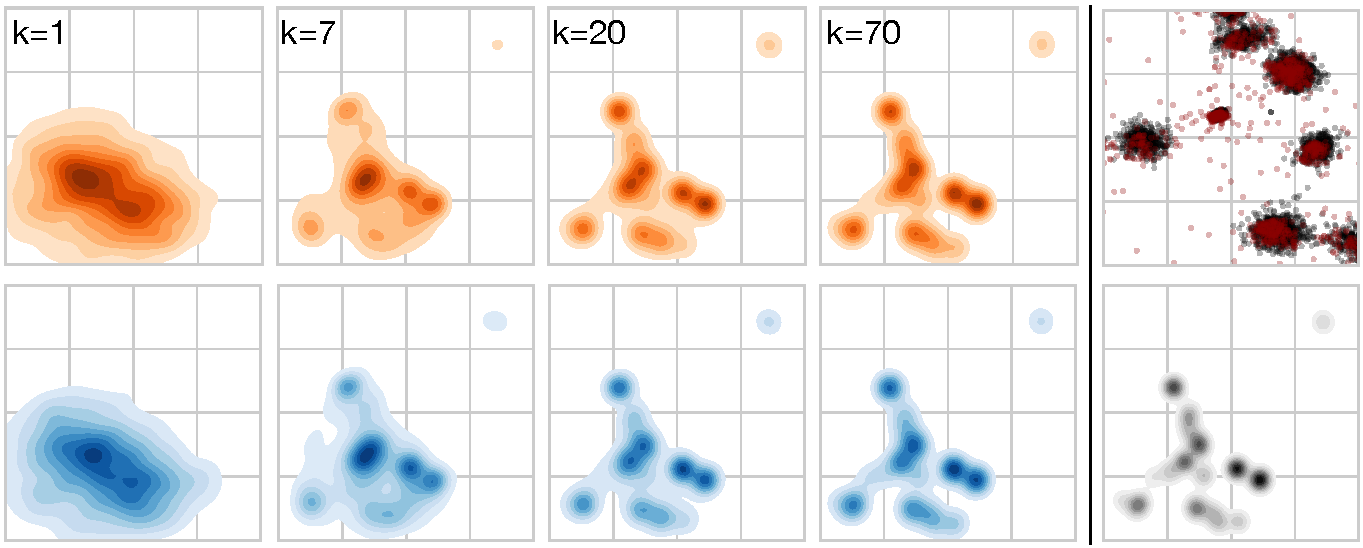
\includegraphics[width=0.685\columnwidth]{figures/gmm_iter.pdf}
	\label{fig:toy_example}
} \hfill
\subfigure[]{ 
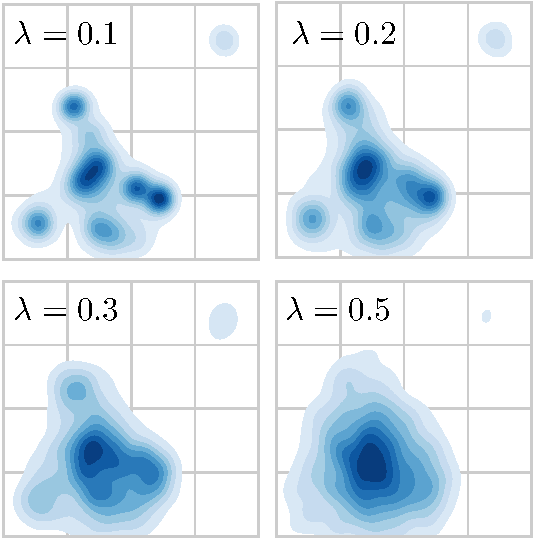
\includegraphics[width=0.268\columnwidth]{figures/gmm_reg.pdf}
\label{fig:lambda_supp}
 }
\caption{a) Toy example. training data $y_i$ consists in $50 000$ samples drawn from a Gaussian Mixture Model with $20$ components of random weights, covariances and locations. \textbf{Left:} Output distribution for learning (top) and testing (bottom) particles. \textbf{Right:} (top) Close-up of some generated samples in red superimposed with learning points in black. (bottom) Target distribution. $N_\theta=30$, $N=3000$, $h=1$, $\lambda=10^{-4}$. b) Influence of the regularization parameter $\lambda$. The higher $\lambda$, the more entropic the output distribution.}
\end{figure}

In this section, we evaluate the proposed SWF Algorithm~\ref{algo:flow} on different datasets. In all cases, the $N$ initial particles $\bar{X}^i_0\in\mathbb{R}^d$ are obtained by first drawing i.i.d. $\bar{Z}^i\in\mathbb{R}^r$ with $r\leq d$, each one with i.i.d standard Gaussian entries. Then we take $\bar{X}^i_0=A\bar{Z}^i$ with $A$ being a random $d\times r$ matrix. This results in a proposal distribution $\mu=\mathcal{N}(0,AA^\star)$. This procedure allows to have an arbitrary input dimension and yet use SWF.

\subsection{Toy example: multivariate Gaussian Mixture Model}
\label{sub:toy_example}

\begin{wrapfigure}{R}{0.42\textwidth}
\begin{centering}
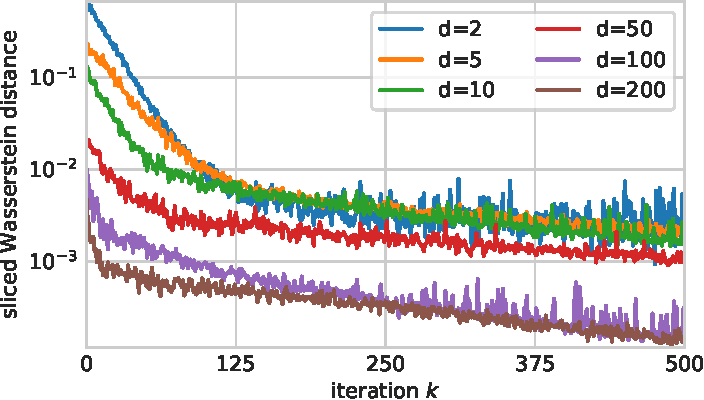
\includegraphics[width=0.42\columnwidth]{figures/SW2_cost-crop.pdf}
\par\end{centering}
\caption{Approximately computed $\SW$ between output $\bar{\mu}_{k}^{N}$ and data distributions $\nu$ in the toy example GMM case for different data dimensions $d$.
\label{fig:toy_sw}}
\end{wrapfigure}
We first illustrate SWF on a toy example. We randomly drew the parameters for a GMM with $20$ components and various dimensions $d$. The weights of the components were drawn randomly, as well as their covariance matrices and centroids. In all draws, the first centroid was sent far from the other ones (multiplied by $3$) so as to test the model for mode collapse.



% \begin{figure}
% \begin{subfigure}[t]{0.5\textwidth}
% \begin{centering}
% \setlength\tabcolsep{1pt}
% \begin{tabular}{ccc|c}
% $k=1$ & $k=7$ & $k=70$ & target\tabularnewline
% 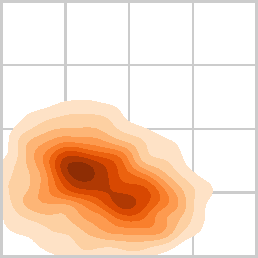
\includegraphics[width=2cm]{figures/toy_save/output_dist_k=1-crop.pdf} & 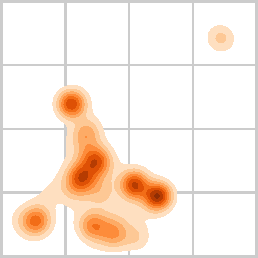
\includegraphics[width=2cm]{figures/toy_save/output_dist_k=20-crop.pdf} & 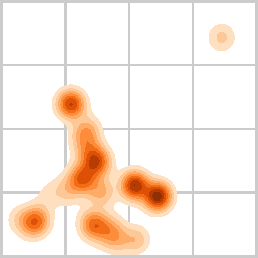
\includegraphics[width=2cm]{figures/toy_save/output_dist_k=70-crop.pdf} &  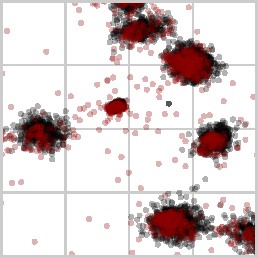
\includegraphics[width=2cm]{figures/scatter_output_particles_k=70-crop.pdf}\tabularnewline
% 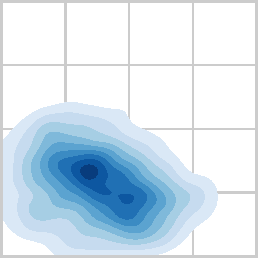
\includegraphics[width=2cm]{figures/toy_load/output_dist_k=1-crop.pdf} & 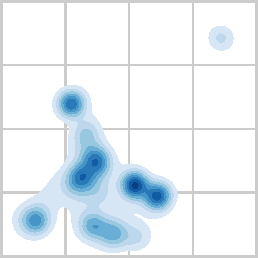
\includegraphics[width=2cm]{figures/toy_load/output_dist_k=20-crop.pdf} & 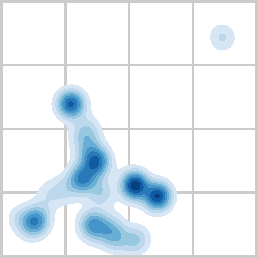
\includegraphics[width=2cm]{figures/toy_load/output_dist_k=70-crop.pdf} &  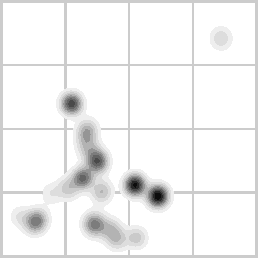
\includegraphics[width=2cm]{figures/target-crop.pdf}\tabularnewline
% \end{tabular}
% % \par
% \end{centering}
% \caption{Toy example.}
% \label{fig:toy_example}
% \end{subfigure}
% \end{figure}

% \begin{figure}
% \begin{centering}
% \setlength\tabcolsep{1pt}
% \begin{tabular}{cccccc}
% $\lambda=0$ & $\lambda=0.1$ & $\lambda=0.2$ & $\lambda=0.3$ & $\lambda=0.5$ & $\lambda=1$\tabularnewline
% 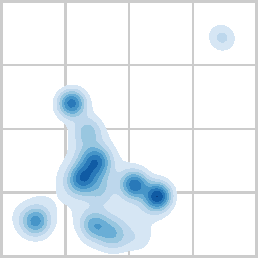
\includegraphics[width=2cm]{figures/supplementary/regularization/r0_output_dist_k=70-crop.pdf} & 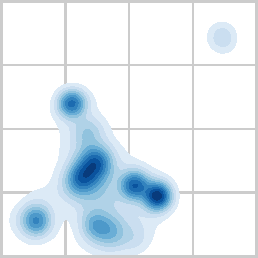
\includegraphics[width=2cm]{figures/supplementary/regularization/r01_output_dist_k=70-crop.pdf} & 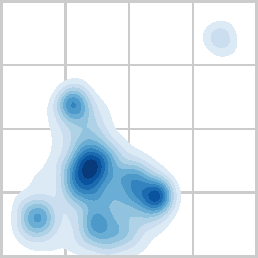
\includegraphics[width=2cm]{figures/supplementary/regularization/r02_output_dist_k=70-crop.pdf} &  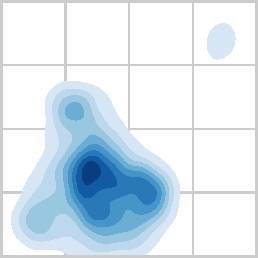
\includegraphics[width=2cm]{figures/supplementary/regularization/r03_output_dist_k=70-crop.pdf}&  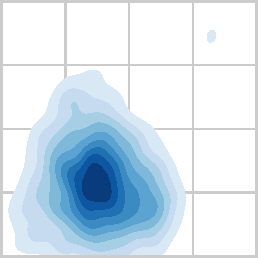
\includegraphics[width=2cm]{figures/supplementary/regularization/r05_output_dist_k=70-crop.pdf} &  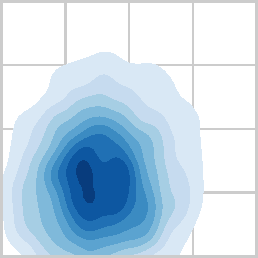
\includegraphics[width=2cm]{figures/supplementary/regularization/r1_output_dist_k=70-crop.pdf}
% \end{tabular}
% \par
% \end{centering}
% \caption{Influence of the regularization parameter $\lambda$. The higher $\lambda$, the more entropic the output distribution.\label{fig:lambda_supp}}
% \end{figure}








% \newcommand{\ww}{0.2}


% \begin{minipage}{\linewidth}
% \begin{minipage}{0.4\textwidth}
% \begin{figure}[H]
% \centering
% \begin{tabular}{ccc|c}
% $k=1$ & $k=7$ & $k=70$ & target\tabularnewline
% 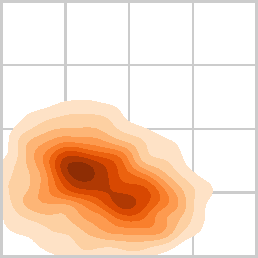
\includegraphics[width=0.1\columnwidth]{figures/toy_save/output_dist_k=1-crop.pdf} & 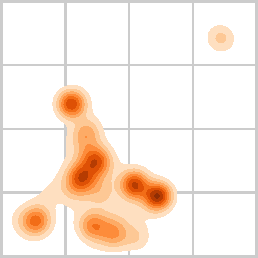
\includegraphics[width=0.1\columnwidth]{figures/toy_save/output_dist_k=20-crop.pdf} & 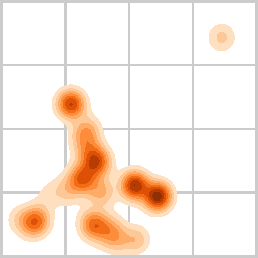
\includegraphics[width=0.1\columnwidth]{figures/toy_save/output_dist_k=70-crop.pdf} &  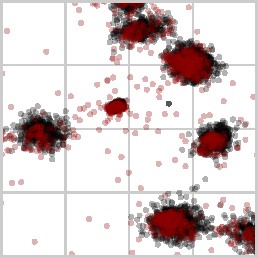
\includegraphics[width=0.1\columnwidth]{figures/scatter_output_particles_k=70-crop.pdf}\tabularnewline
% 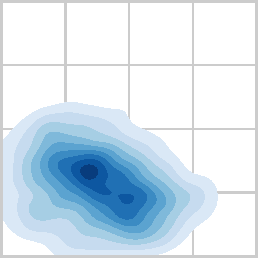
\includegraphics[width=0.1\columnwidth]{figures/toy_load/output_dist_k=1-crop.pdf} & 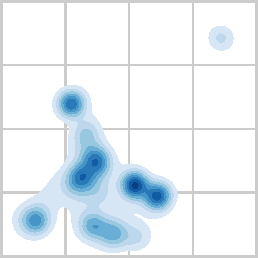
\includegraphics[width=0.1\columnwidth]{figures/toy_load/output_dist_k=20-crop.pdf} & 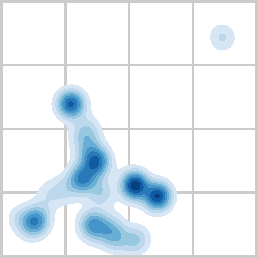
\includegraphics[width=0.1\columnwidth]{figures/toy_load/output_dist_k=70-crop.pdf} &  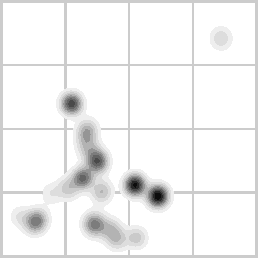
\includegraphics[width=0.1\columnwidth]{figures/target-crop.pdf}\tabularnewline
% \end{tabular}
% \par
% \caption{Toy example: training data $y_i$ consists in $50 000$ samples drawn from a Gaussian Mixture Model with $20$ components of random weights, covariances and locations. \textbf{Left:} Output distribution for learning (top) and testing (bottom) particles. \textbf{Right:} (top) Close-up of some generated samples in red superimposed with learning points in black. (bottom) Target distribution. $N_\theta=30$, $N=3000$, $h=1$, $\lambda=10^{-4}$.
% \label{fig:toy_example}}
% \end{figure}
% \end{minipage}
% %
% \begin{minipage}{0.49\textwidth}
% \begin{figure}[H]
% \centering
% \begin{tabular}{cccc|c}
% $k=2K$ & $k=20K$ & $k=10K$ & $k=40K$ & target\tabularnewline
% 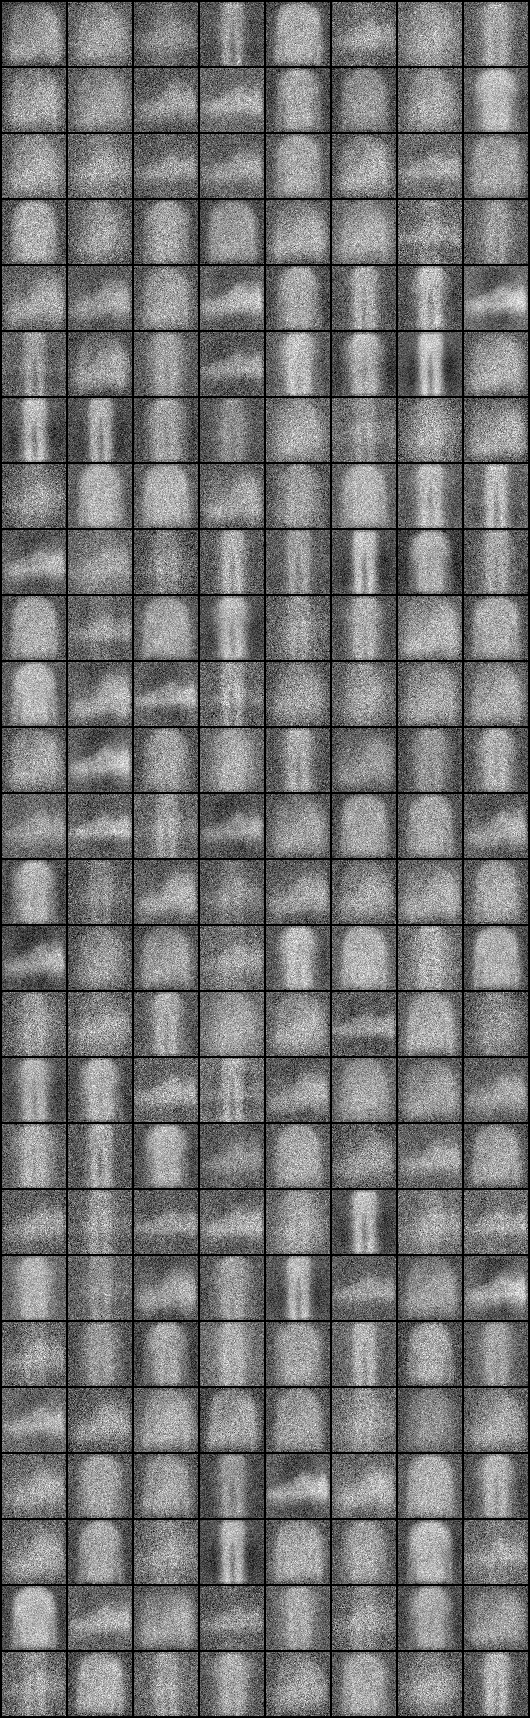
\includegraphics[width=\ww\columnwidth]{figures/FashionMNIST/image_200} & 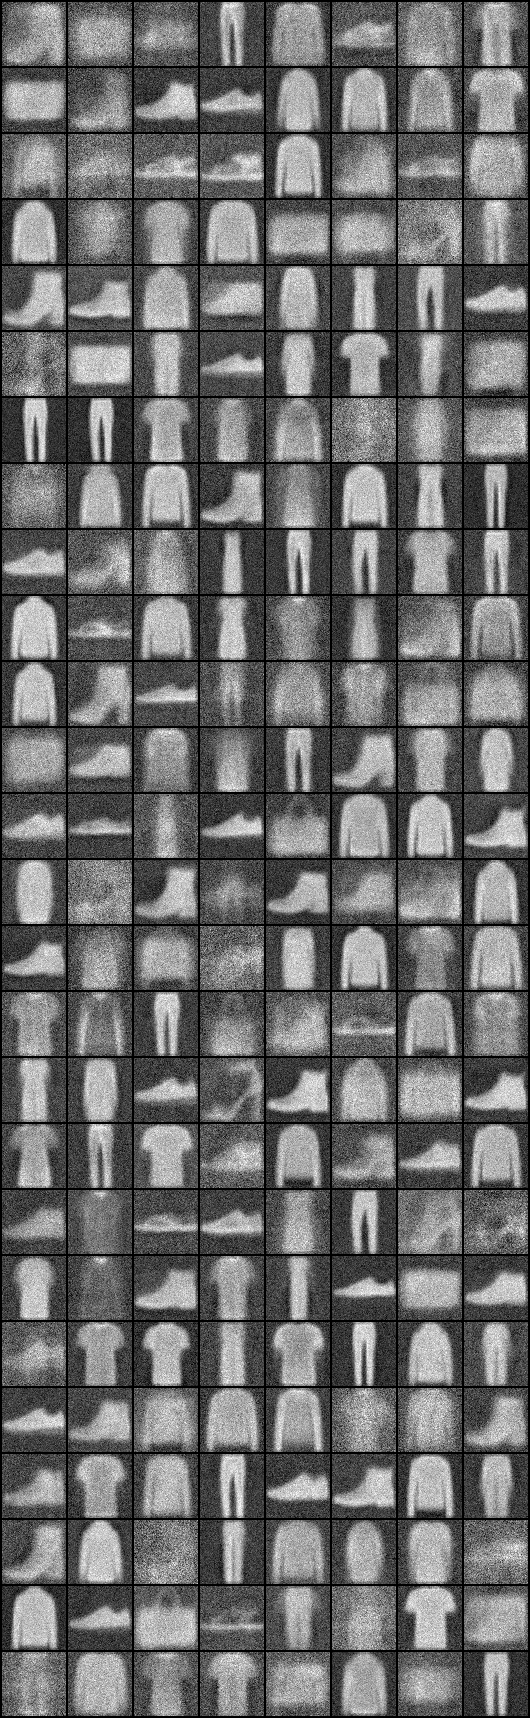
\includegraphics[width=\ww\columnwidth]{figures/FashionMNIST/image_2000} & 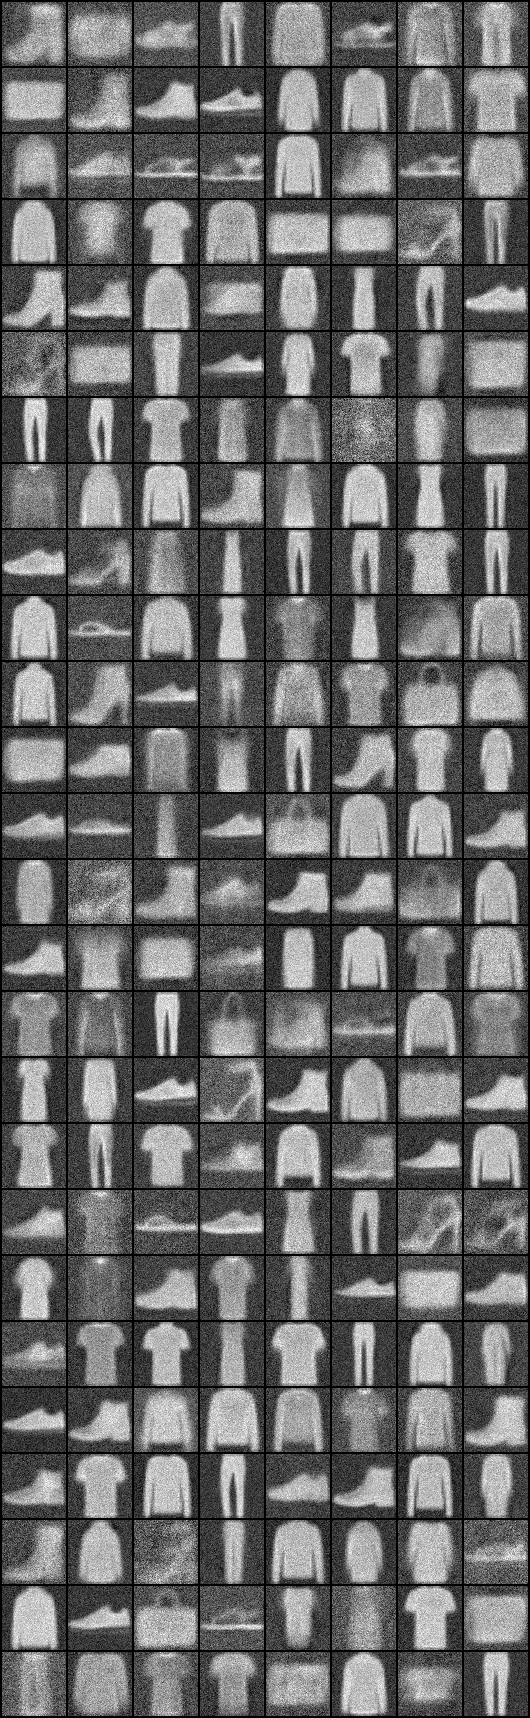
\includegraphics[width=\ww\columnwidth]{figures/FashionMNIST/image_10000} & 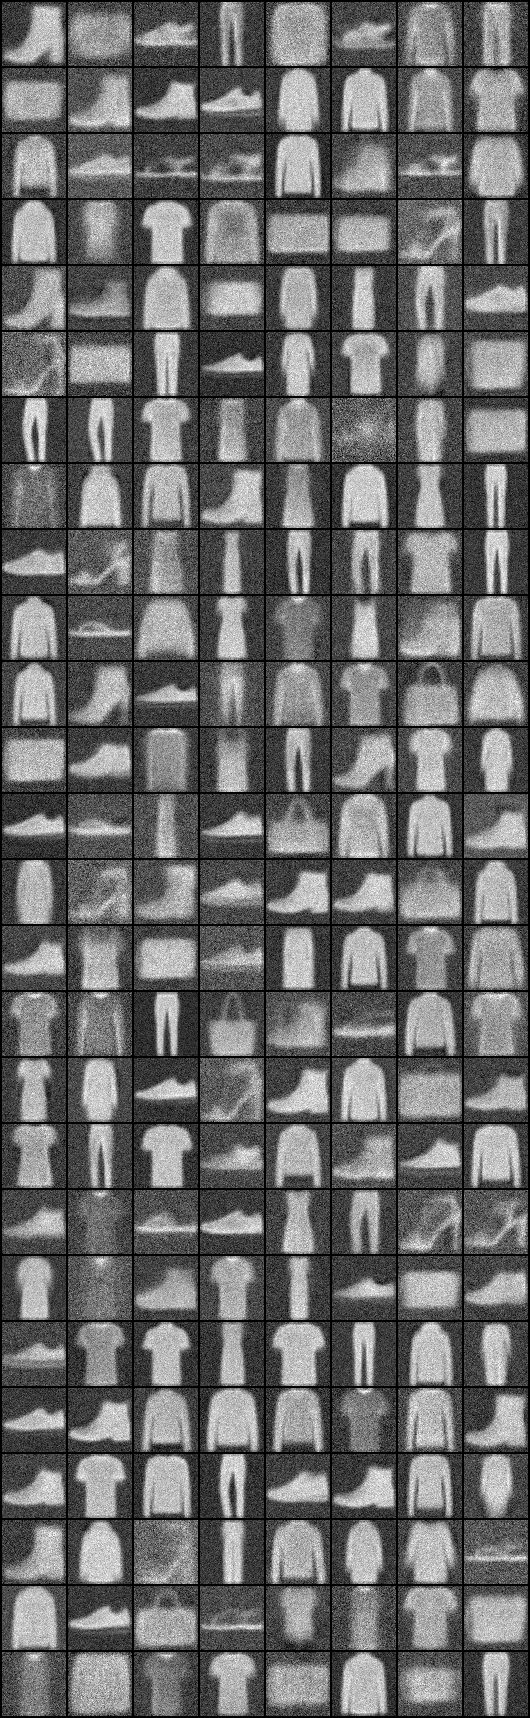
\includegraphics[width=\ww\columnwidth]{figures/FashionMNIST/image_38400} & 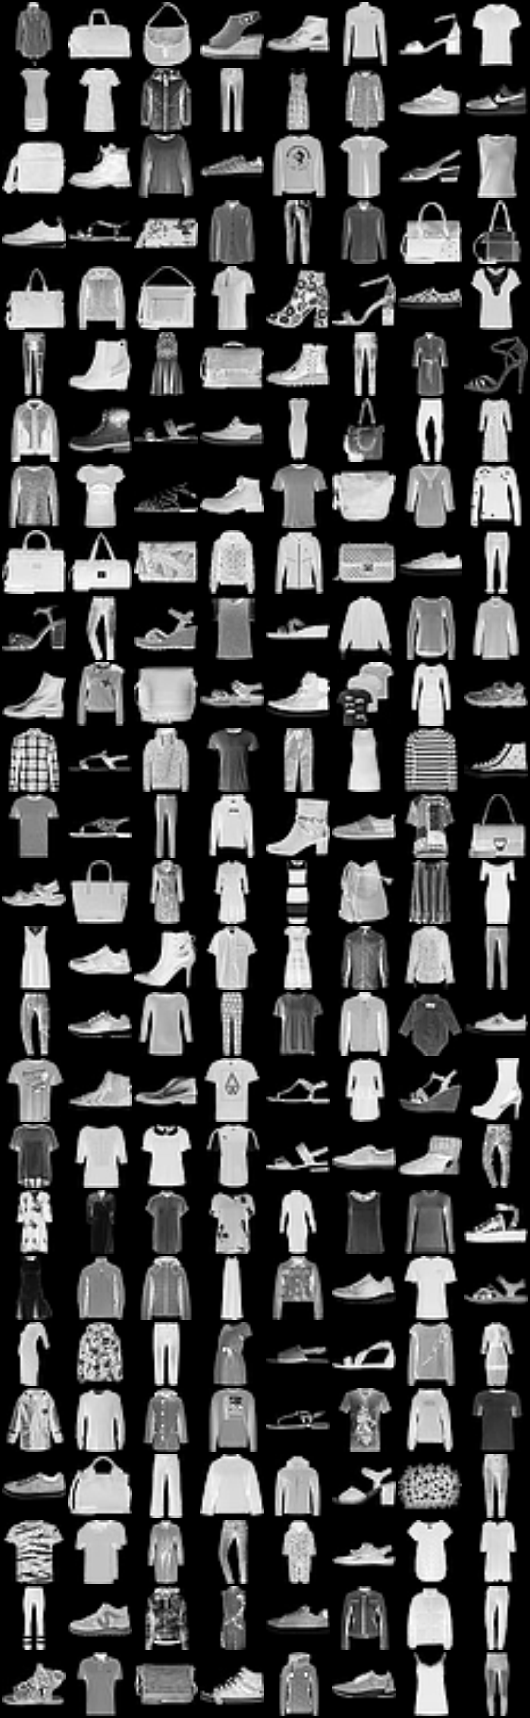
\includegraphics[width=\ww\columnwidth]{figures/FashionMNIST/dataset_example}\tabularnewline
% \end{tabular}
% \par
% \caption{Applying SWF on the Fashion MNIST dataset.
% \label{fig:fashionmnist}}
% \end{figure}
% \end{minipage}
% \end{minipage}



Our first experiment is to assess whether SWF achieves its objective of decreasing the sliced Wasserstein distance between the output $\bar{\mu}_{k}^{N}$ and the target $\nu$. For each run, this is done by computing \label{eqn:sw} using an empirical average over random directions $\theta\in\Sp^{d-1}$ and the analytical expression \eqref{eq:W1D} for the scalar Wasserstein distance. In Figure~\ref{fig:toy_sw}, we see a steady decrease of the cost for all runs, as predicted by the theory presented above.

Then, we illustrate the generating power of the model with one particular such example, depicted on Figure~\ref{fig:toy_example}. There, the target distribution is displayed on the rightmost panel, as obtained through a contour plot of the data samples. On the left panel, we see the output distribution of the SWF at different iterations. As can be seen, the output converges rapidly to the target. Furthermore, we can see that the QF $F^{-1}_{\theta^*_\#\bar{\mu}_{kh}^{N}}$ computed with one set of particles (so-called \textit{training} stage) can perfectly be reused for new unseen particles in a subsequent \textit{test} stage. In any case, two remarkable things may be seen on this figure. First, even when some modes lie far away from the others, SWF is able to generate them successfully and we never observed mode collapse. This is due to the OT nature of the procedure. Second, the genenerated samples do not reproduce the learning data, which is in particular enforced by the regularization term $\lambda$.




\subsection{Experiments on real data}
\label{sub:real_data}

In a second set of experiments, we tested the SWF for implicit generative modeling of larger more challenging datasets than our GMM toy example. Here, we report the results we obtained on the recently proposed FashionMNIST dataset \cite{xiao2017fashion}, that is advocated as much more challenging than the traditional MNIST, although also featuring $50000$ training samples that are gray-scale images, dispatched into $10$ classes\footnote{Results for MNIST can be found in the supplementary material for this paper.}. All images were interpolated as $64\times 64$, yielding $d=4096$. $h=300$, $\lambda=10^{-6}$, $N_\theta=200$



\begin{figure}
\centering
\subfigure[]{
\includegraphics[width=0.55\columnwidth]{figures/fmnist2.pdf}
\label{fig:fashionmnist}	
}\hfill
\subfigure[]{
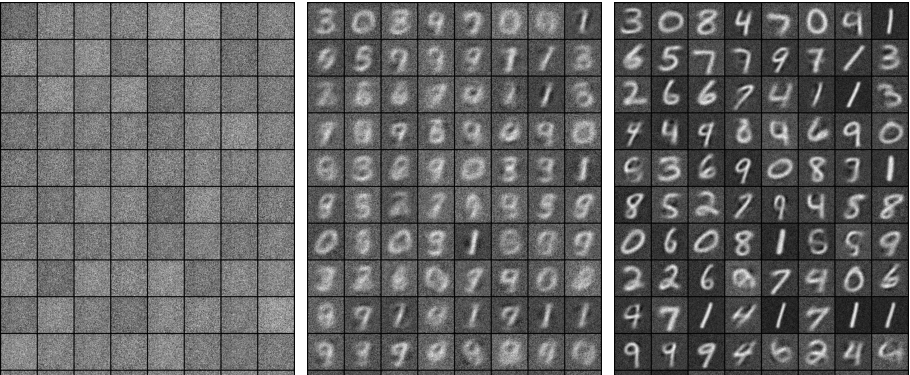
\includegraphics[width=0.41\columnwidth]{figures/mnist.pdf}
\label{fig:fashionmnist}	
}
\caption{Applying SWF on the Fashion MNIST dataset.}
\end{figure}

% \begin{figure}
% \begin{centering}
%   \setlength\tabcolsep{1pt}

% \begin{tabular}{cccc|c}
% $k=200$ & $k=2000$ & $k=10000$ & $k=40000$ & target\tabularnewline
% 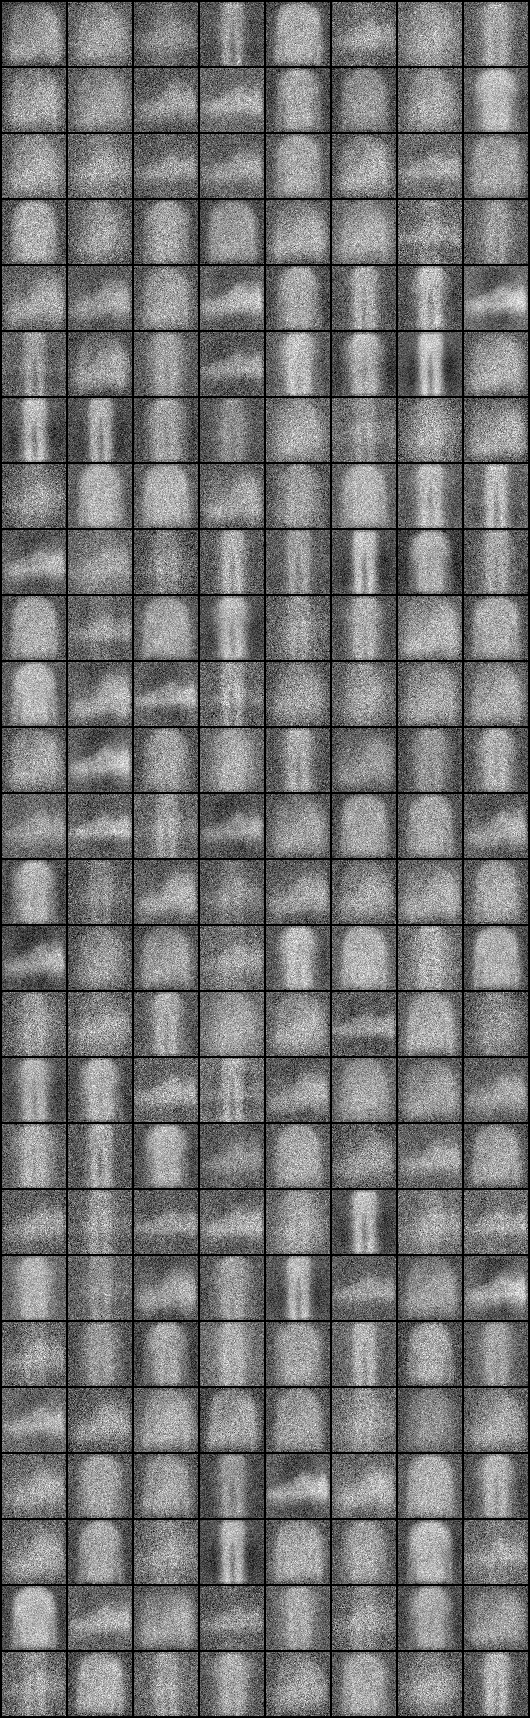
\includegraphics[height=6cm]{figures/FashionMNIST/image_200} & 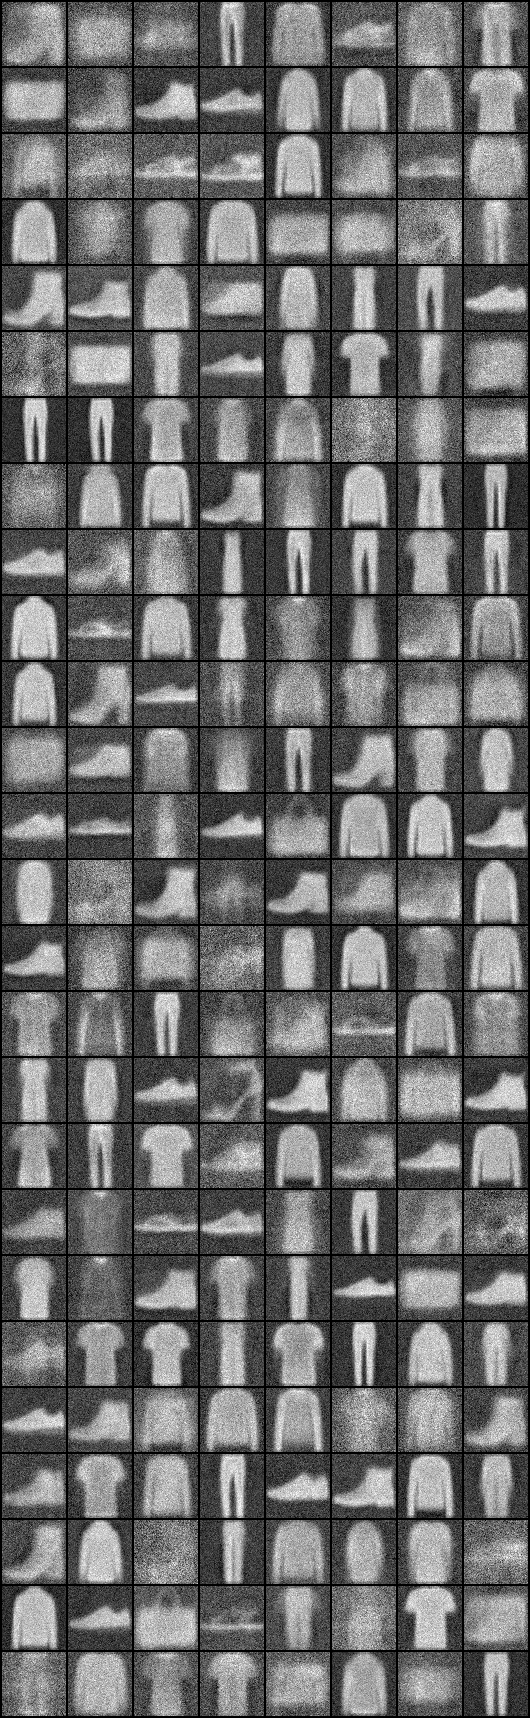
\includegraphics[height=6cm]{figures/FashionMNIST/image_2000} & 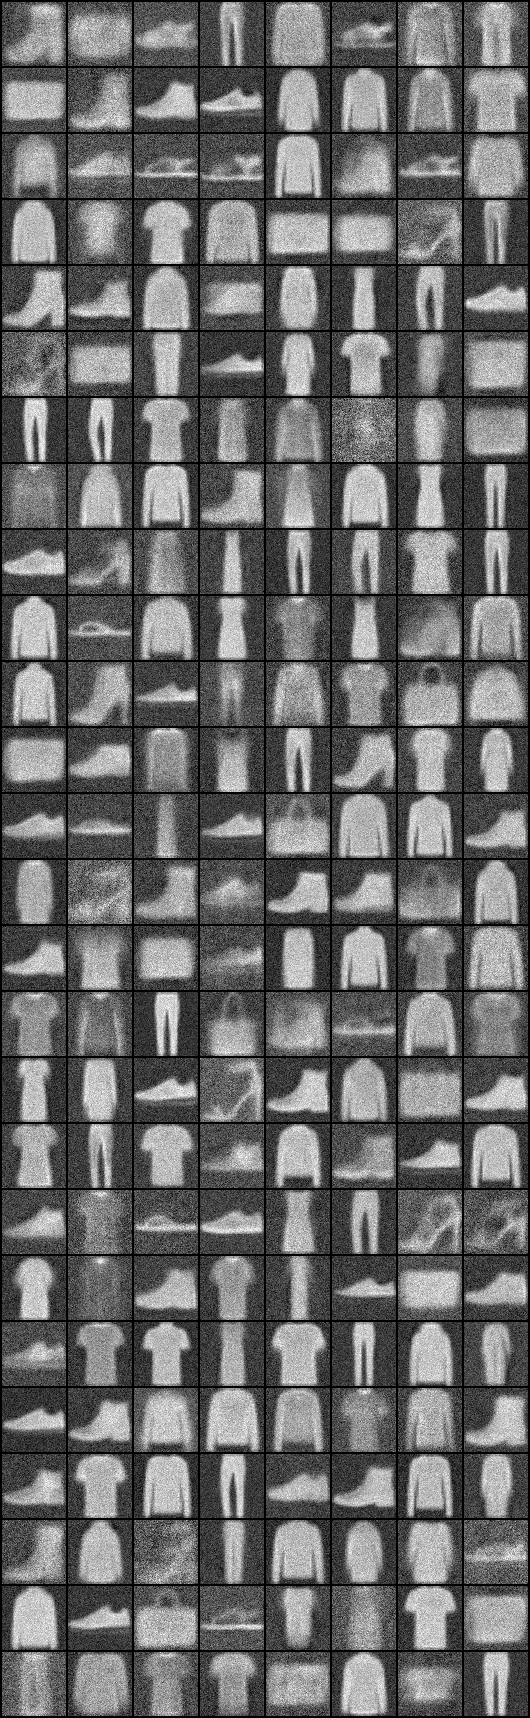
\includegraphics[height=6cm]{figures/FashionMNIST/image_10000} & 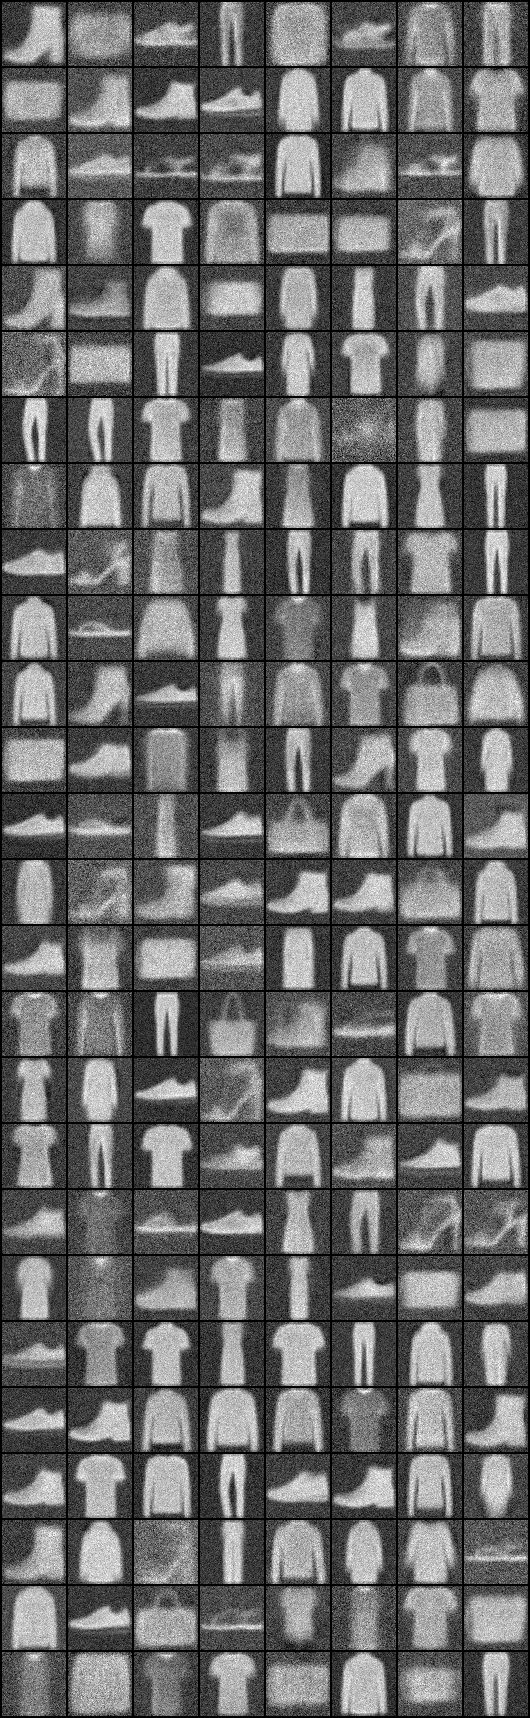
\includegraphics[height=6cm]{figures/FashionMNIST/image_38400} & 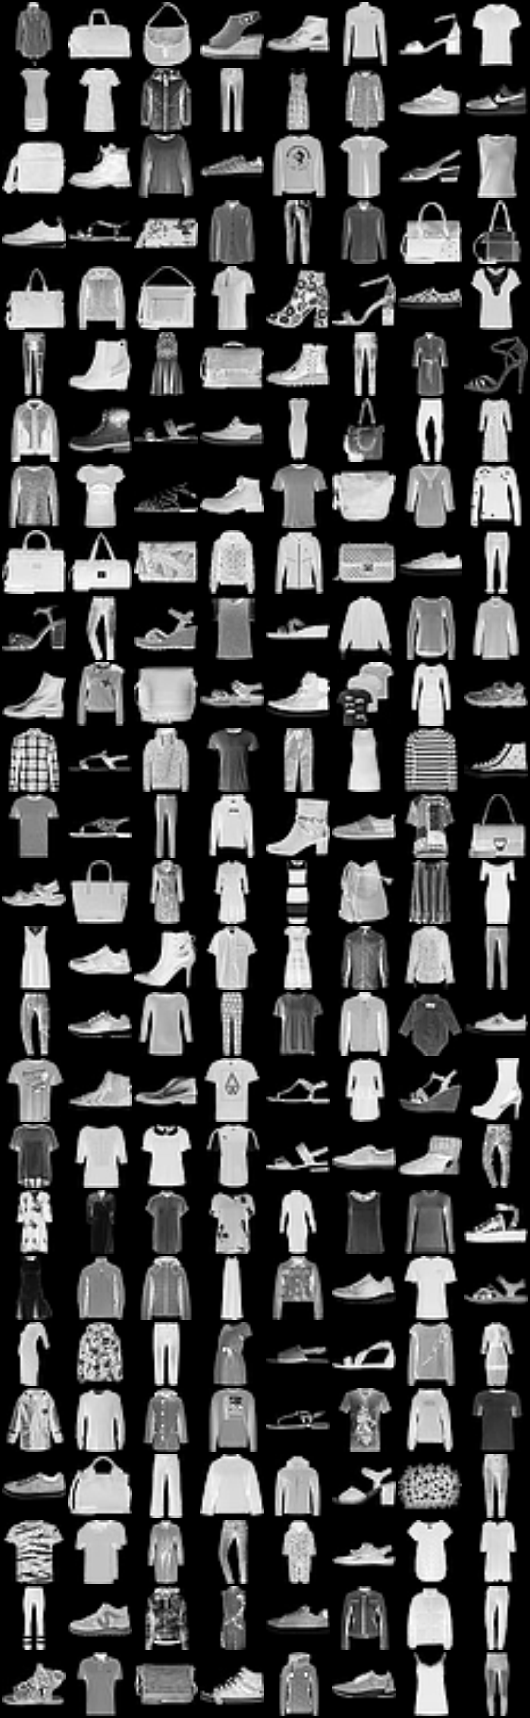
\includegraphics[height=6cm]{figures/FashionMNIST/dataset_example}\tabularnewline
% \end{tabular}
% \par\end{centering}
% \caption{Applying SWF on the Fashion MNIST dataset.\label{fig:fashionmnist}}
% \end{figure}

On figure \ref{fig:fashionmnist}, we can see that a few thousand iterations of SWF is sufficient to get generated samples that capture most features of the training data. We note however that we are currently missing generation of fine-grained textures. We also display the SW2 loss of this run along iterations. Interestingly, such an experiment requires around $1h$ of computing power for a laptop computer on CPU, to be compared with the important ressources required by many other generative models.

% \end{itemize}




\section{Conclusion}



\bibliography{./references.bib}
\bibliographystyle{unsrt}



\end{document}
